\documentclass[10pt]{article}
\usepackage[letterpaper,margin=.8in]{geometry}
\usepackage{amsmath,amssymb,booktabs,graphicx,hyperref,xurl,float}
\emergencystretch=2em
\hypersetup{hidelinks}\graphicspath{{../figures/}}\setlength{\parskip}{4pt}
\title{S28-A and Original S27-C: Joint Mechanism Evidence}
\author{Completed registered execution record}\date{24 November 2026}
\begin{document}\maketitle
\section{Execution and Scientific Questions}
Starting from the S28-0 commit \texttt{de7d010}, explicit user authorization activates six BN-by-GELU control fits (A), followed by twelve fresh four-Source/one-held-RX fits (C). Both original JSON plans remain byte-identical. All eighteen fits complete 200 epochs. C is launched unconditionally with its original splits and seeds; all A Dev and C held inference is delayed until both complete cohorts are sealed and committed. No A outcome changes a C decision.

A asks whether the contribution of three tokenizer GELUs depends on three middle BN modules. C asks whether higher held accuracy coincides with a smaller Source-to-held loss. These questions and decisions are distinct; shared data and development history do not create statistically independent datasets. No S28-B, IQ-only, ASK Strict-IB, seed replacement or architecture search is run. After this report, the remaining automatic scientific fit budget is zero.
\section{A: All Four Cells and the Registered Interaction}
\begin{center}\small\begin{tabular}{lrrrrrr}\toprule
Arm&Params&Dev acc.&Fit SD&Macro-F1&Worst RX&Source acc.\\\midrule
H0&133,690&97.335&0.552&97.326&93.667&98.175\\
LA&133,690&96.583&0.779&96.554&90.383&97.742\\
H2&133,338&96.145&0.454&96.135&94.100&97.142\\
H2\_LA&133,338&96.743&0.703&96.728&91.633&97.808\\
LP&138,346&94.500&1.831&94.423&88.333&96.358\\
\bottomrule\end{tabular}\end{center}
H0 keeps BN/GELU; LA removes only the three GELUs; H2 removes only the three BN modules; H2\_LA removes both. LP is a reused secondary Long-Patch comparator. Accuracy/F1 are percentages and SD describes six fold/seed means in pp.
\[
\Delta_{BN\times GELU}=(A_{H0}-A_{LA})-(A_{H2}-A_{H2\_LA}).
\]
The primary interaction is +1.350pp, conditional RX 95\% interval [0.930,1.750]. 5/6 paired effects share its direction. Fold means are +0.977 and +1.723pp. The registered two-sided practical rule is met.
The GELU benefit is larger with middle BN under this complete training procedure.
The unchanged rule requires magnitude at least .5pp, a conditional interval excluding zero, at least 5/6 same-direction pairs and both fold means in that direction. Three seeds are averaged within each of ten unique RXs before 10,000 bootstrap repetitions, seed 28028. The intervals condition on the observed seeds, packets and architecture choices; they do not include fresh-acquisition or selection uncertainty or multiplicity-corrected confirmatory claims.
\clearpage
\begin{figure}[H]\centering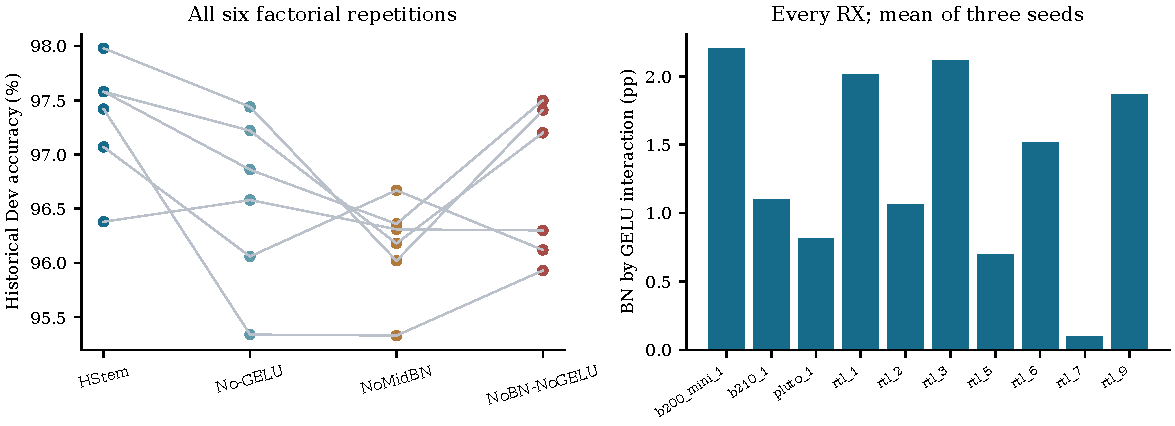
\includegraphics[width=.98\linewidth]{A_interaction.pdf}
\caption{All paired A accuracies and every RX interaction, including counterexamples.}\end{figure}
\section{A: Simple Effects and Causal Limits}
\begin{center}\small\begin{tabular}{lrr}\toprule
Descriptive contrast&Mean(pp)&Conditional 95\% RX interval\\\midrule
GELU\_with\_BN&+0.752&[0.197,1.432]\\
GELU\_without\_BN&-0.598&[-1.150,0.168]\\
BN\_with\_GELU&+1.190&[0.750,1.563]\\
BN\_without\_GELU&-0.160&[-0.472,0.125]\\
H2\_LA\_minus\_LP&+2.243&[1.863,2.588]\\
\bottomrule\end{tabular}\end{center}
The two shared-stem BN modules, two LeakyReLUs and MHA remain. Removing middle BN removes 352 affine parameters and changes batch statistics, running statistics and the optimization trajectory jointly. The intervention compares complete training procedures, not a unique normalization or factorization cause. LP still differs in grouping, free parameters, initialization and computation. Source validation already selects checkpoints. Simple effects, absolute Source learning and the factorial interaction must be read together; secondary contrasts do not replace the primary rule.
With BN present, GELU adds .752pp on average; without BN its mean effect is -.598pp, with a conditional interval crossing zero. The latter does not by itself establish harm from GELU. The double-removal model still reaches 96.743\% and exceeds LP by 2.243pp on average; all six paired differences are positive. Thus these BN/GELU interventions do not exhaust the observed LP difference; that residual still cannot uniquely identify factorized parameterization as the cause.
\clearpage
\section{C: Absolute Held Performance and Gap Reduction}
The original fold 0 training RXs are rtl1/rtl3/rtl6/rtl9 with b210\_1 held; fold 1 trains b200\_mini\_1/pluto\_1/rtl2/rtl7 with rtl\_5 held. Fresh H0/LP use the fixed S27C-H4x160 seed domain and 6,400/1,600 train/validation packets. No five-RX checkpoint is loaded. Only the four training RXs choose checkpoints; all 2,000 held packets are evaluated after all twelve C models seal.
\[
G=A_{\rm SourceVal}-A_{\rm Held},\qquad\Delta G=G_{H0}-G_{LP}.
\]
\begin{center}\small\begin{tabular}{lrrr}\toprule
Held RX&Source H0-LP(pp)&Held H0-LP(pp)&$\Delta G$(pp)\\\midrule
b210\_1&+2.146&+4.583&-2.437\\
rtl\_5&+1.042&+1.383&-0.342\\
\bottomrule\end{tabular}\end{center}
The original consistent-pilot rule is not met. 5/6 pairs simultaneously have positive held improvement and negative gap difference. Across six repeats, mean held improvement is +2.983pp, Source improvement +1.594pp and gap difference -1.390pp.
The unchanged rule additionally requires held improvement at least .5pp and $\Delta G\leq-.5$pp in both RX/fold means. A smaller gap alone is insufficient if held identification is worse. Source ceilings can distort gaps. Two held RXs do not become six independent receiver units: no population-RX significance or bootstrap is reported. Higher held accuracy without stable gap reduction supports stronger overall discrimination, rather than an established RX-specific suppression mechanism.
All six held-accuracy differences favor HStem. Mean HStem/LP held accuracy is 89.367/84.783\% on b210\_1 and 95.167/93.783\% on rtl\_5. The rtl\_5 gap reduction is .342pp, below the frozen .5pp threshold; it remains a favorable mean direction, without passing the registered criterion. The b210\_1 seed 202 counterexample improves held accuracy by 1.150pp but improves Source by 2.000pp, enlarging the gap by .850pp. Neither the threshold nor this repeat is changed after evaluation.
\begin{figure}[H]\centering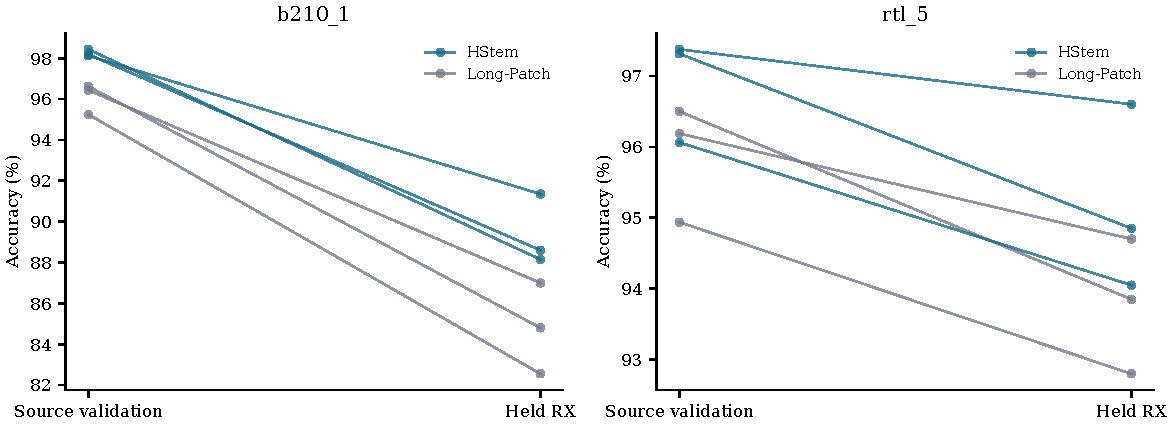
\includegraphics[width=.98\linewidth]{C_source_held.pdf}
\caption{All twelve new C models, Source validation to held accuracy. Both RXs and all seeds remain visible.}\end{figure}
\clearpage
\section{C: Every Paired Repeat and Fixed Diagnostics}
\begin{center}\small\begin{tabular}{rrrrrrrr}\toprule
Fold&Seed&H0 Source&H0 Held&LP Source&LP Held&Held diff.&$\Delta G$\\\midrule
0&201&98.188&88.600&96.625&84.800&+3.800&-2.237\\
0&202&98.438&88.150&96.438&87.000&+1.150&+0.850\\
0&203&98.125&91.350&95.250&82.550&+8.800&-5.925\\
1&201&97.375&96.600&96.188&94.700&+1.900&-0.713\\
1&202&97.312&94.850&96.500&93.850&+1.000&-0.188\\
1&203&96.062&94.050&94.937&92.800&+1.250&-0.125\\
\bottomrule\end{tabular}\end{center}
\begin{figure}[H]\centering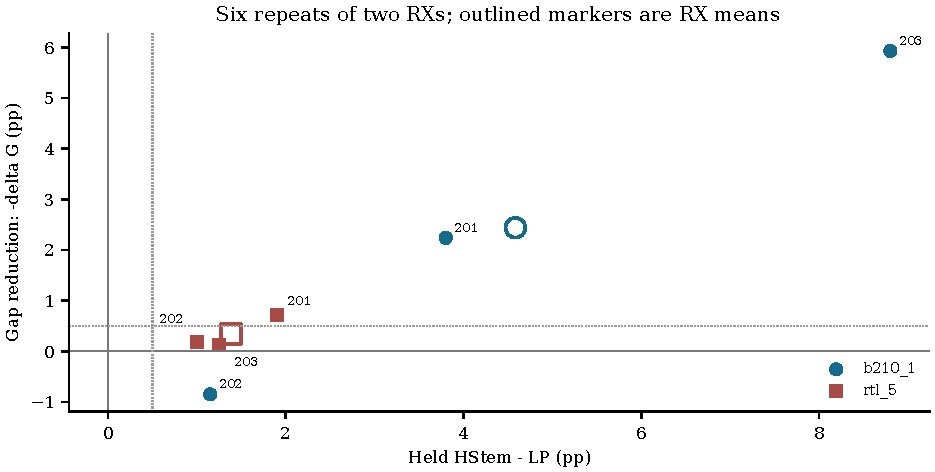
\includegraphics[width=.80\linewidth]{C_gap_pairs.pdf}
\caption{Held accuracy gain and gap reduction jointly. Outlined points are means of the same two RX units, not new independent observations.}\end{figure}
All C models use three predeclared 64D taps: tokenizer mean, pre-backend mean and final classifier input. Pooling precedes per-packet L2 normalization. Source geometry uses all 1,600 validation packets, 40/TX/RX; held geometry uses only the original last 40/TX, 400 packets, while classification uses all 2,000 held packets. All 72 layer records and 72,000 vectors remain saved. All layers, normalization, class errors, CE/F1 and true-class margins are retained.

Held-only geometry has a single RX; conditional across-RX scatter is zero by construction. Its $J_c$ is marked not identifiable and the algebraic epsilon ratio is saved separately, without an invariance interpretation. $J_w$, scatter and margins are descriptive: Source selected the checkpoints, Source/Held RX counts differ, and jointly trained representations do not establish causal information flow. S27-B's counterexample to a sufficient final-$J_w$ explanation remains valid.
With unit-normalized packets, let $B$ be TX-centroid scatter about the global centroid, $D$ the TX/RX-centroid scatter about each TX centroid, and $W$ the packet scatter within TX/RX cells. Balanced cell averages retain the S25 definitions $J_c=B/(D+10^{-12})$ and $J_w=B/(D+W+10^{-12})$; the latter denominator includes both receiver-centroid and within-cell dispersion.

All three-seed layer means are retained below; held $J_c$ is undefined and omitted.
\begin{center}\scriptsize\begin{tabular}{llrrrrrr}\toprule
Fold&Tap&Source $J_c$ H0&LP&Source $J_w$ H0&LP&Held $J_w$ H0&LP\\\midrule
0&tokens&46.244&10.585&1.414&0.220&1.607&0.486\\
0&pre\_backend&104.697&83.685&4.525&3.229&5.206&4.122\\
0&final&68.179&57.593&6.712&4.901&6.455&4.772\\
1&tokens&8.923&9.312&0.589&0.355&0.729&0.383\\
1&pre\_backend&21.926&27.113&1.573&2.127&1.872&2.505\\
1&final&29.250&26.619&4.573&4.410&6.296&6.054\\
\bottomrule\end{tabular}\end{center}
In fold 1 at the pre-backend tap, HStem has lower Source $J_c$, Source $J_w$ and held $J_w$ than LP, despite higher mean held accuracy. The same fold also has slightly lower tokenizer Source $J_c$. Higher final $J_w$ in both folds does not erase these counterexamples or prove monotonic receiver-information removal.
\section{Precision and Research History}
S28-0 established a finite affine tokenizer only conditional on the shared nonlinear stem and frozen evaluation BN, with explicit first/last-token corrections. Its native TF32 runtime failed the original tolerance and changed 1/12000 predictions. The separate TF32-off 300-packet probe qualified numerical export; it did not replace that failure or the historical recipe. This execution trains original architectures in the original FP32-tensor/matmul-TF32-off/cuDNN-TF32-on mode, never materialized substitutes.

All receiver data have development history. A uses the historical five-Source protocol, including physical RXs later held from the distinct freshly fitted C models. C is a Source-internal held-RX pilot; it is not a new independent acquisition or blind test. No unknown-TX rejection or security attack claim follows from closed-set accuracy.
\section{Every New Fit, Training Cost and Audit}
\begin{center}\small\begin{tabular}{llrrrrr}\toprule
Stage&Arm/Fold/Seed&Best ep.&Source CE&Source acc.&Updates&Wall(s)\\\midrule
A&H2\_LA/0/201&186&0.07434&97.650&25000&1832.5\\
A&H2\_LA/0/202&186&0.07428&98.100&25000&1837.2\\
A&H2\_LA/0/203&165&0.07013&98.050&25000&1915.7\\
A&H2\_LA/1/201&190&0.07447&98.000&25000&1909.6\\
A&H2\_LA/1/202&171&0.08178&97.200&25000&1838.7\\
A&H2\_LA/1/203&191&0.07339&97.850&25000&1841.8\\
C&H0/0/201&173&0.05771&98.188&20000&1448.4\\
C&LP/0/201&193&0.10421&96.625&20000&1501.7\\
C&H0/0/202&192&0.05291&98.438&20000&1370.1\\
C&LP/0/202&154&0.09426&96.438&20000&1458.2\\
C&H0/0/203&177&0.06037&98.125&20000&1377.7\\
C&LP/0/203&169&0.14871&95.250&20000&1452.9\\
C&H0/1/201&192&0.08554&97.375&20000&1351.5\\
C&LP/1/201&159&0.10917&96.188&20000&1412.2\\
C&H0/1/202&142&0.08919&97.312&20000&1351.1\\
C&LP/1/202&125&0.10203&96.500&20000&1404.1\\
C&H0/1/203&171&0.11257&96.062&20000&1347.1\\
C&LP/1/203&152&0.14194&94.937&20000&1226.1\\
\bottomrule\end{tabular}\end{center}
All eighteen fits run 200 epochs without early stopping, reseeding or target-driven tuning. A has 125 updates/epoch; C has 100, yielding 390,000 retained updates. Atomic full-epoch snapshots include current and best models, optimizer, all RNG states and history. Any discarded partial-epoch work after a pause is not counted as retained updates. Summed fit wall times overlap under isolated CUDA workers and are not exclusive GPU hours. Engineering synthetic updates are counted separately from scientific fits.
\begin{figure}[H]\centering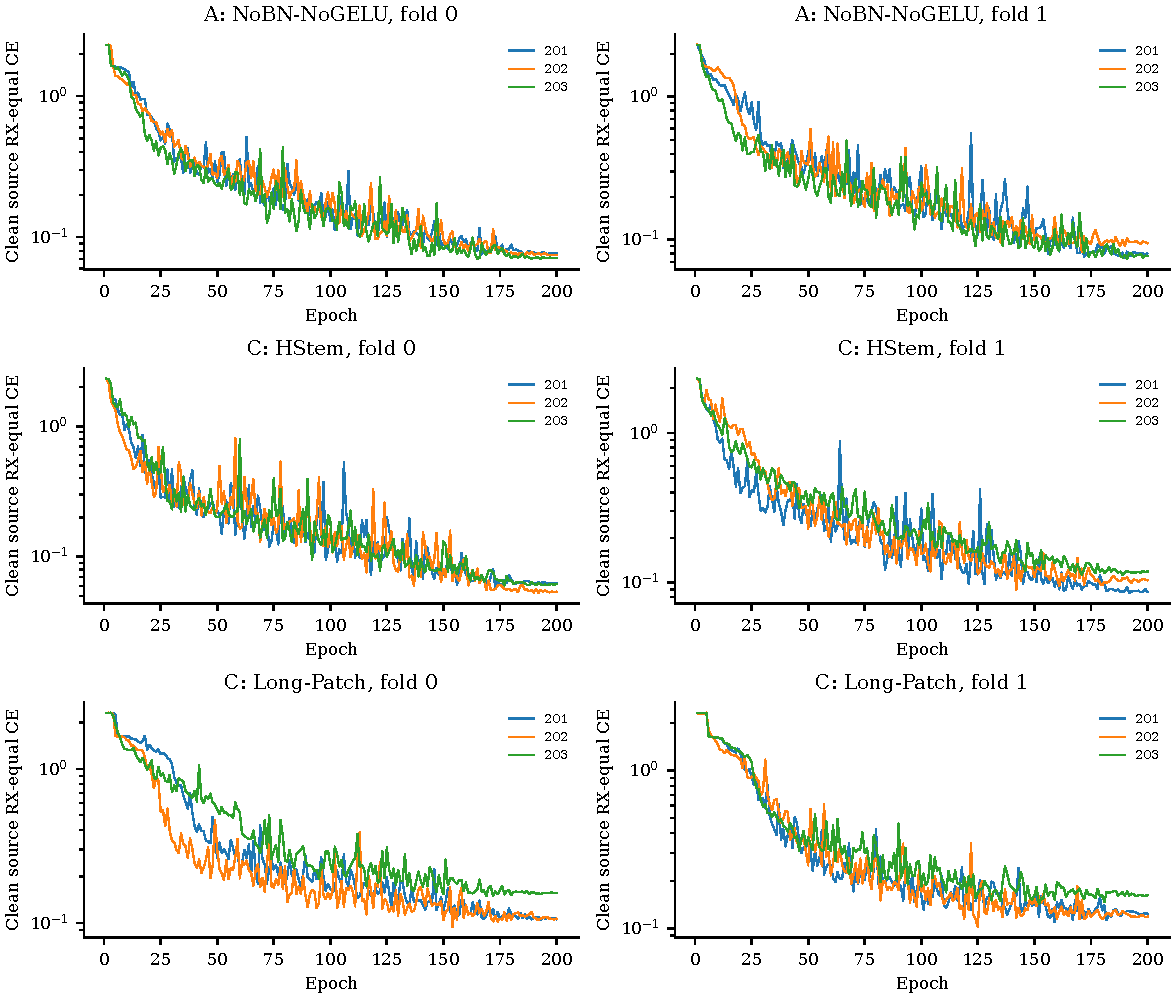
\includegraphics[width=.98\linewidth]{all_training.pdf}
\caption{Every new source-CE trajectory, all 18 fits and all 200 epochs.}\end{figure}
\clearpage
\section{Evidence Boundaries and Stop}
A supports a signed interaction of the selected BN/GELU training procedures.
C does not meet its joint two-RX criterion; absolute discrimination and receiver-specific gap reduction must remain distinct.
Neither outcome uniquely identifies factorized optimization or physical receiver invariance. The evidence matrix updates the completed A/C claims while retaining previous mathematical, preprocessing and historical-data limits. No favorable result automatically rewrites TIFS contributions. The remaining automatic fitting budget is zero. Any future same-function factorized-versus-direct optimization study needs matched boundary constraints, freedom, initialization and optimizer-state auditing; no S28-B arm is started here.
\section{Reproduction and Integrity}
The activation, original plans, engineering gate, seeds, permissions and execution hashes were committed and pushed before Source IO. A 5-RX uses 8,000/2,000 packets and P-H5x160 seeds; C 4-RX uses 6,400/1,600 and the frozen new seed domain. Minimum clean Source RX-equal CE alone selects checkpoints. Data order/noise and surviving initialization pairings are checked. Both complete cohort seals precede every new Dev/held read.

The independent audit recomputes metrics from 324,000 saved target and 79,200 Source predictions, all C geometry, the A conditional interaction and C gap rule. It separately reruns all eighteen new models on permitted Source validation and restores their saved logits exactly. It checks all 200-epoch histories, best-source checkpoints, actual RF streams and hashes. Twenty-four old A baseline models reproduce archived Dev logits elementwise; their weights/configurations/histories remain unchanged. No Confirm/blind data or target adaptation is introduced. Larger waveforms, checkpoint snapshots and per-packet arrays stay local; code, full logs, aggregate tables and audit records are published.

After all eighteen models sealed, the first evaluation encountered a filename/payload argument-name collision in prediction saving, before any Dev or held read. A separate committed IO-only wrapper changed only that storage parameter, preserving all original files, errors, models, formulas and plans. A synthetic writer fixture passed and the same sealed cohort continued; no scientific fit or optimizer step was repeated by the repair. The original and recovery logs and hashes are retained.

The Chinese report supplies all numerical contrasts, per-RX/TX tables, limitations and next-step recommendations. The task stops at this complete registered evidence record, without extra fits or independent-generalization certification.
\end{document}
